\documentclass[12pt,a4paper]{amsart}

\usepackage[T1]{fontenc}
\usepackage[utf8]{inputenc}
\usepackage[slovene]{babel}
\usepackage{amsmath}
\usepackage{amssymb}
\usepackage{amsthm}
\usepackage{graphicx}

\textwidth 15cm
\textheight 24cm
\oddsidemargin.5cm
\evensidemargin.5cm
\topmargin-5mm
\addtolength{\footskip}{10pt}
\pagestyle{plain}

\usepackage{algorithm}
\usepackage{algpseudocode}
\renewcommand{\algorithmicrequire}{\textbf{Vhod:}}
\renewcommand{\algorithmicensure}{\textbf{Izhod:}}
\makeatletter
\renewcommand{\ALG@name}{Algoritem}
\makeatother

\theoremstyle{definition} % tekst napisan pokoncno
\newtheorem{definicija}{Definicija}[section]
\newtheorem{primer}[definicija]{Primer}
\newtheorem{opomba}[definicija]{Opomba}
\newtheorem{zgled}[definicija]{Zgled}

\theoremstyle{plain} % tekst napisan posevno
\newtheorem{lema}[definicija]{Lema}
%\newtheorem{zgled}[definicija]{Zgled}
\newtheorem{izrek}[definicija]{Izrek}
\newtheorem{trditev}[definicija]{Trditev}
\newtheorem{posledica}[definicija]{Posledica}

%\usepackage{graphicx}
\newtheorem{theorem}{Theorem}[section]
\newtheorem{definition}{Definicija}[section]
\newtheorem{corollary}{Posledica}[theorem]
\newtheorem{lemma}[theorem]{Lema}

\newcommand{\program}{Finančna matematika} 
\newcommand{\imeavtorja}{Lina Ivanova, Tia Krofel} 
\newcommand{\naslovdela}{Bernsteinovi bazni polinomi treh spremenljivk}
\newcommand{\letnica}{2023} 

\title{Bernstainovi baznih polinomov treh spremenljivk}
\author{Tia Krofel, Lina Ivanova}
\date{December 2023}

\begin{document}

% od tod do povzetka ne spreminjaj nicesar
\thispagestyle{empty}
\noindent{\large
UNIVERZA V LJUBLJANI\\[1mm]
FAKULTETA ZA MATEMATIKO IN FIZIKO
%\program\ -- 1.~stopnja
}
\vfill

\begin{center}{\large
\imeavtorja\\[2mm]
{\bf \naslovdela}\\[10mm]
Seminar pri predmetu Računalniško podprto (geometrijsko) oblikovanje\\[1cm]
%Mentorica: \imementorja
}
\end{center}
\vfill

\noindent{\large
Ljubljana, 2023}
\pagebreak

\section{Uvod}
V tem delu seminarja predstavimo Bernsteinove bazne polinome 
treh spremenljivk. Najprej predstavimo prostor polinomov,
kjer lahko operiramo s polinomi treh spremenljivk. Nato si ogledamo 
baricentrične koordinate za poljubno točko $(x,y,z)$ in kako izgleda 
kontrolna mreža, ki je v obliki strukture iz tetraedrov.
Zatem definiramo naslovni pojem, torej Bernsteinove bazne polinome 
treh spremenljivk, čemur sledi poglavje o Bernsteinovi formi polinomov 
treh spremenljivk. Za konec izpišemo še de Casteljaujev algoritem 
in si ogledamo smerne odvode vektorjev, ki so elementi prostora $\mathbb{R}^3$.

\section{Prostor $\mathbb{P}_d$}

Za začetek s $\mathbb{P}_d$ označimo prostor polinomov treh spremenljivk stopnje $d$, 
torej prostor končnih dimenzij z vsemi funkcijami oblike 

$$ p(x,y,z):=\sum_{0\leq i+j+k\leq d}a_{ijk}x^iy^jz^k,$$

kjer $a_{ijk}\in\mathbb{R}$.

\begin{lema}
    Dimenzija prostora $\mathbb{P}_d$ je enaka $\binom{d+3}{3}$,
    medtem ko monomi $\{x^iy^jz^k\}$ tvorijo bazo. 
\end{lema}

\begin{proof}
    Po definiciji monomi $\{x^iy^jz^k\}$ razpenjajo
    prostor $\mathbb{P}_d$.
    Linearna neodvisnost pa sledi, če enačimo
    $p(x,y,z)=\sum_{0\leq i+j+k\leq d}a_{ijk}x^iy^jz^k=0$
    in vidimo, da to velja natanko tedaj, ko 
    $a_{ijk}=0$ za vse $0\leq i+j+k\leq d$.
\end{proof}

V nadaljevanju bomo za parcialne odvode funkcij treh spremenljivk po 
$x,y$ in $z$ uporabljali oznake $D_x,D_y,D_z$.
Obenem naj velja $D^\alpha := D^{\alpha_1}_xD^{\alpha_2}_yD^{\alpha_3}_z$,
kjer je $\alpha := (\alpha_1,\alpha_2,\alpha_3)$ vektor nenegativnih 
celih števil, red odvoda $D^{\alpha}$ pa je enak $|\alpha| := \alpha_1+\alpha_2+\alpha_3$.\\


\section{Baricentrične koordinate}

\begin{definicija}
  Naj bo $T$ tetraeder z ogli"s"ci $\textbf{V}_{i} = (x_{i}, y_{i}, z_{i})$, kjer $i \in \{1, 2, 3, 4\}$, ozna"cen s
  $T = \langle\textbf{V}_{1}, \textbf{V}_{2}, \textbf{V}_{3}, \textbf{V}_{4}\rangle.$
  
  \begin{figure}[h!]
    \centering
    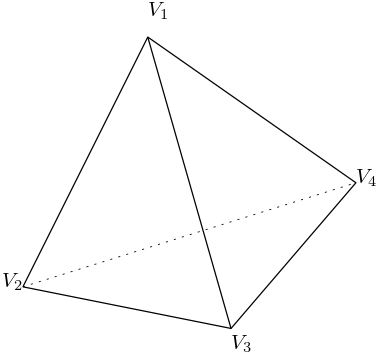
\includegraphics[scale=0.4]{tetraedar}
    \caption{Baricentri"cne koordinate kot razmerje.}
    \label{fig:tetraedar}
  \end{figure}
\end{definicija}

\begin{lemma}
Vsako to"cko $\textbf{V} = (x, y, z) \in \mathbb{R}$  lahko na enoli"cen na"cin zapi"semo kot kombinacijo oblike
\begin{equation*}
\textbf{V} = u_{1}\textbf{V}_{1} + u_{2}\textbf{V}_{2} + u_{3}\textbf{V}_{3} + u_{4}\textbf{V}_{4},
\end{equation*}
kjer je
$$
u_{1} + u_{2} + u_{3} + u_{4} = 1.
$$
\end{lemma}
\begin{proof}
Ena"cbe $(x, y, z) = u_{1}(x_{1}, y_{1}, z_{1}) + u_{2}(x_{2}, y_{2}, z_{2}) + u_{3}(x_{3}, y_{3}, z_{3}) + u_{4}(x_{4}, y_{4}, z_{4}) $ in $u_{1} + u_{2} + u_{3} + u_{4} = 1$ lahko zapi"semo v matri"cni obliki kot
$$
\begin{bmatrix}
  1 & 1 & 1 & 1\\ 
  x_{1} & x_{2} & x_{3} & x_{4}\\
  y_{1} & y_{2} & y_{3} & y_{4}\\
  z_{1} & z_{2} & z_{3} & z_{4}
\end{bmatrix}
\begin{bmatrix}
u_{1}\\
u_{2}\\
u_{3}\\
u_{4}
\end{bmatrix}
=
\begin{bmatrix}
1\\
x\\
y\\
z
\end{bmatrix}
$$
in ozna"cimo
$$
A = \begin{bmatrix}
  1 & 1 & 1 & 1\\ 
  x_{1} & x_{2} & x_{3} & x_{4}\\
  y_{1} & y_{2} & y_{3} & y_{4}\\
  z_{1} & z_{2} & z_{3} & z_{4}
\end{bmatrix}.
$$
Re"sitev tega sistema je enoli"cna natanko tedaj, ko je $det(A) \neq 0$. Velja, da je $det(A) = 6V(T)$, kjer je $pl(T)$ volumen tetraedra $T$. Torej mora veljati
$$
det(A) = 6V_{T} \neq 0.
$$
S pomočjo Cramerjevega pravila dobimo
$$
u_{1} = \frac{1}{det(A)}
\begin{vmatrix}
  1 & 1 & 1 & 1\\ 
  x & x_{2} & x_{3} & x_{4}\\
  y & y_{2} & y_{3} & y_{4}\\
  z & z_{2} & z_{3} & z_{4}
\end{vmatrix}
=
\frac{pl(\langle\textbf{V}, \textbf{V}_{2}, \textbf{V}_{3}, \textbf{V}_{4}\rangle)}{pl(\langle\textbf{V}_{1}, \textbf{V}_{2}, \textbf{V}_{3}, \textbf{V}_{4}\rangle)}
$$
in podobno 
$$
u_{2} = \frac{pl(\langle\textbf{V}_{1}, \textbf{V}, \textbf{V}_{3}, \textbf{V}_{4}\rangle)}{pl(\langle\textbf{V}_{1}, \textbf{V}_{2}, \textbf{V}_{3}, \textbf{V}_{4}\rangle)}
$$
\vspace{2mm}
$$
u_{3} = \frac{pl(\langle\textbf{V}_{1}, \textbf{V}_{2}, \textbf{V}, \textbf{V}_{4}\rangle)}{pl(\langle\textbf{V}_{1}, \textbf{V}_{2}, \textbf{V}_{3}, \textbf{V}_{4}\rangle)}
$$
\vspace{2mm}
$$
u_{4} = \frac{pl(\langle\textbf{V}_{1}, \textbf{V}_{2}, \textbf{V}_{3}, \textbf{V}\rangle)}{pl(\langle\textbf{V}_{1}, \textbf{V}_{2}, \textbf{V}_{3}, \textbf{V}_{4}\rangle)}
$$
\end{proof}
To"cke $(u_{1}, u_{2}, u_{3}, u_{4})$ tvorijo baricentri"cne koordinate neke poljubne to"cke $\textbf{V} = (x, y, z)$ glede na tetraeder $T$. 
Njihove lastnosti so podobne lastnostim baricentričnih koordinat, povezanih s trikotniki v primeru dveh spremenljivk. 
Zgornja lema nam v resnici pove, da $u_{1}$ predstavlja razmerje med prostornino tetraedra $\langle\textbf{V}, \textbf{V}_{2}, \textbf{V}_{3}, \textbf{V}_{4}\rangle$ 
in prostornino $T$ - podobno pa velja tudi za ostale tri to"cke $u_{2}, u_{3}$ in $u_{4}$. 

V nadaljevanje bomo ozna"cevali $\textbf{u} = (u_{1}, u_{2}, u_{3}, u_{4})$. 

\subsection{Domenske to"cke}
Naj bodo $\textbf{u}$ baricentri"cne koordinate poljubne to"cke $(x, y, z)$ 
glede na izbran tetraeder $T = \langle\textbf{V}_{1}, \textbf{V}_{2}, \textbf{V}_{3}, \textbf{V}_{4}\rangle$. 
Domenske to"cke Bézierjevega polinoma lahko definiramo kot
$$
\textbf{X}_{\textbf{i}} = \frac{i}{n}\textbf{V}_{1} + \frac{j}{n}\textbf{V}_{2} + \frac{k}{n}\textbf{V}_{3} + \frac{l}{n}\textbf{V}_{4}
$$
za vsak $\textbf{i} = (i, j, k, l)$, kjer $|\textbf{i}| = n$. 
Baricentrične koordinate domenske točke 
$\textbf{X}$ označimo kot $Bar(\textbf{X}_{\textbf{i}}; T) = \xi^{T}_{\textbf{i}}$.\\

\begin{figure}[h!]
\centering
  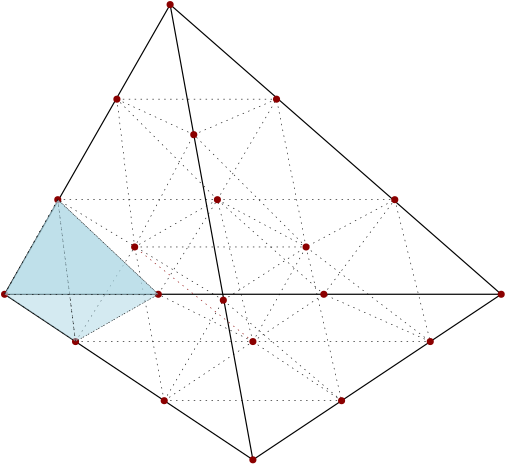
\includegraphics[scale=0.4]{domen}
  \caption{Domenske to"cke}
  \label{fig:domenske}
\end{figure}

\section{Bernstainovi baznih polinomov treh spremenljivk}

\begin{izrek}
  Naj bo $T$ tetraeder in $b_1,b_2,b_3,b_4$
  baricentrične koordinatne funkcije.
  Potem definiramo Bernsteinov bazni polinom treh spremenljivk 
  stopnje $d$ glede na $T$ kot 

  $$
  B_{ijkl}^d := \frac{d!}{i!\text{ }j!\text{ }k!\text{ }l!}b_1^ib_2^jb_3^kb_4^l,\text{    }i+j+k+l=d.
  $$
\end{izrek}

Ob pojavu negativnih indeksov je $B_{ijkl}^d$ povsod enak 0.
Ker so $b_1,b_2,b_3,b_4$ linearni polinomi, sledi,
da je vsak $B_{ijkl}^d$ polinom stopnje $d$. 

\begin{izrek}
  Množica $\mathcal{B}^d := \{B_{ijkl}^d\}_{i+j+k+l=d}$
  Bernsteinovih baznih polinomov predstavlja bazo 
  prostora polinomov treh spremenljivk $\mathbb{P}_d$.
  Še več,

  $$
  \sum_{i+j+k+l=d}B^d_{ijkl}(v)=1\text{ }\forall v\in\mathbb{R}^3
  $$
  
  in

  $$
  0\leq B_{ijkl}^d(v)\leq 1\text{ }\forall v\in T.
  $$
\end{izrek}

\begin{proof}
  Bernsteinovi bazni polinomi res tvorijo razčlenitev enote, saj velja

  $$
  1 = (b_1+b_2+b_3+b_4)^d = \sum_{i+j+k+l=d}\frac{d!}{i!\text{ }j!\text{ }k!\text{ }l!}b_1^ib_2^jb_3^kb_4^l.
  $$

  Če sedaj pomnožimo $x=b_1x_1+b_2x_2+b_3x_3+b_4x_4$ z
  $1 = \sum_{i+j+k+l=d-1}B_{ijk}^{d-1}$ in enako naredimo za 
  $y$ in $z$, dobimo:

  $$
  x = \sum_{i+j+k+l=d}\frac{(ix_1+jx_2+kx_3+lx_4)}{d}B_{ijkl}^d(x,y,z),
  $$
  $$
  y = \sum_{i+j+k+l=d}\frac{(iy_1+jy_2+ky_3+ly_4)}{d}B_{ijkl}^d(x,y,z),
  $$
  $$
  z = \sum_{i+j+k+l=d}\frac{(iz_1+jz_2+kz_3+lz_4)}{d}B_{ijkl}^d(x,y,z).
  $$

  Z indukcijo pokažemo, da so vsi monomi 
  $\{x^\nu y^\mu z^\kappa\}_{0\leq \nu+\mu+\kappa\leq d}$
  v obsegu $\mathcal{B}^d$.

  Ker je število baznih funkcij v $\mathcal{B}^d$ enako 
  dimenziji $\mathbb{P}_d$, tj. $\binom{d+3}{2}$, sledi, da  
  $\mathcal{B}^d$ predstavlja bazo $\mathbb{P}_d$.
  
  Iz tega, da so $b_1,b_2,b_3,b_4$ nenegativne za $v\in T$, sledi,
  da imajo $B_{ijkl}^d$ to isto lastnost. 

  Potem $\sum_{i+j+k+l=d}B_{ijkl}^d(v)=1\text{ }\forall v\in\mathbb{R}^3$ 
  direktno implicira zadnjo neenakost, in sicer $B_{ijkl}^d(v)\leq1$.
\end{proof}

\section{Bernstainova forma polinomov treh spremenljivk}
Vsak polinom treh spremenljivk lahko zapi"semo s pomo"cjo Bernsteinovih baznih polinomov. 
Naj v nadaljevanju $T = \langle\textbf{V}_{1}, \textbf{V}_{2}, \textbf{V}_{3}, \textbf{V}_{4}\rangle$ ustreza naši definiciji tetraedra.  

\begin{corollary}
Vsak polinom $p \in \mathbb{P}^{3}_{n}$ lahko enolično zapišemo v obliki
\begin{equation*} %\label{polinom}
p(\textbf{u}) = \sum_{i + j + k + l = n}c_{ijkl}B^{n}_{ijkl}(\textbf{u}),
\end{equation*}
kjer so $B^{n}_{ijkl}$ Bernsteinovi baznih polinomov glede na tetraeder $T$ in $c_{ijkl}$ Bézierjevi koeficienti.
\end{corollary}

Podano imamo kontrolno mre"zo, ki je v obliki strukture iz tetraedra, kot prikazano na Sliki \ref{fig:kontrolne}. 
Kontrolne to"cke ozna"cimo z $\textbf{b}_{\textbf{i}} = \textbf{b}_{i,j,k,l}$, $|\textbf{i}| = n$. 

\begin{definition}
Bézierjev tetraeder stopnje $n$, dolo"cen s kontrolnimi to"ckami $\textbf{b}_{\textbf{i}}$, $|\textbf{i}| = n$, 
je podan s parametrizacijo
\begin{equation*}
\textbf{p}(\textbf{u}) = \sum_{|\textbf{i}| = n}\textbf{b}_{\textbf{i}}B_{\textbf{i}}^{n}(\textbf{u}),
\end{equation*}
kjer je $\textbf{u} = Bar((x, y, z); T)$.
\end{definition}

\begin{figure}[h!]
\centering
  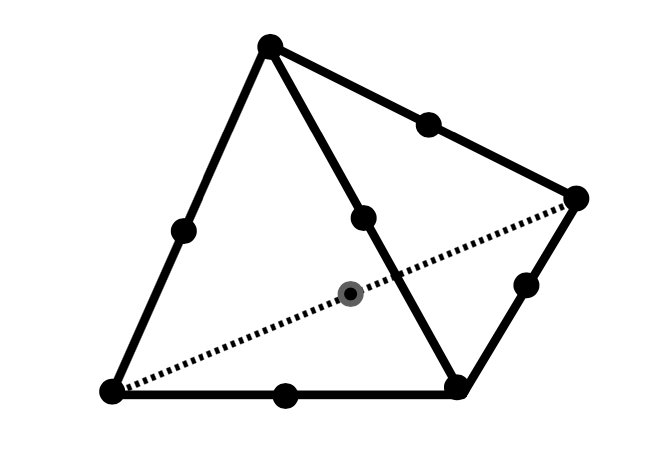
\includegraphics[scale=0.4]{kontrolne.png}
  \caption{Kontrolne to"cke za $n=2$}
  \label{fig:kontrolne}
\end{figure}

\section{De Casteljaujev algoritam}
To"cke na Bézierjevih tetraedrih računamo s pomočjo de Casteljaujevega algoritma, 
ki je posplo"sitev standardnega de Casteljauovega algoritma za Bézierjeve krivulje. 
Vhodni podatki algoritma so kontrolne to"cke $\textbf{b}_{\textbf{i}}$, kjer $|\textbf{i}| = n$ in $i, j, k, l \in \mathbb{N}_{0}$, 
ter to"cka $(x, y, z)$ z baricentri"cnimi koordinatam $\textbf{u} = Bar((x,y,z); T)$. Izhodni podatek tega algoritma je natan"cno to"cka $\textbf{b}_{\textbf{0}}^{n}(\textbf{u})$ na Bezierjevega tetraedra. 

\begin{algorithm}
\caption{de Casteljaujev algoritem}
\begin{algorithmic}
\Require $\textbf{b}_{\textbf{i}}$, $|\textbf{i}| = n,$ $\textbf{i} = (i,j,k,l),$ $i,j,k,l \in \mathbb{N}_{0}$, $\textbf{u} = Bar((x,y,z); T)$
\For{\text{$r = 1, 2, \ldots, n$}}
	\For{$|\textbf{i}| = n-r$}
		\State $\textbf{b}^{r}_{\textbf{i}}(\textbf{u}) = u_{1}\textbf{b}^{r-1}_{\textbf{i}+e_1}(\textbf{u}) + u_{2}\textbf{b}^{r-1}_{\textbf{i}+e_2}(\textbf{u}) + u_{3}\textbf{b}^{r-1}_{\textbf{i}+e_3}(\textbf{u}) + u_{4}\textbf{b}^{r-1}_{\textbf{i}+e_4}(\textbf{u})$
	\EndFor
\EndFor
\Ensure $\textbf{b}_{0,0,0}^{n}(\textbf{u})$
\end{algorithmic}
\end{algorithm}

\section{Odvodi}

Če imamo podan netrivialen vektor $\textbf{u} := (u_x,u_y,u_z) \in \mathbb{R}^3$, 
lahko definiramo smerne odvode funkcije treh spremenljivk $p$ kot 

$$
\left.D_{\textbf{u}}p(x,y,z):=\frac{d}{dt}p(x+tu_x,y+tu_y,z+tu_z)\right|_{t=0}.
$$
\newline
Obenem vemo, da 

$$
D_{\textbf{u}}p(x,y,z) = u_xD_xp(x,y,z)+u_yD_yp(x,y,z)+u_zD_zp(x,y,z),
$$
\newline
kar nakazuje, da je stopnja smernih odvodov polinoma stopnje $d$
enaka $d-1$.
\newline

Naj bo sedaj $T$ tetraeder. Potem $\textbf{u}$ 
opisujejo smerne koordinate $a := (a_1,a_2,a_3,a_4),$
odvisne od $T$, kjer je $a_i := \beta_i-\alpha_i$,
$(\beta_1,\beta_2,\beta_3,\beta_4)$ in $(\alpha_1,\alpha_2,\alpha_3,\alpha_4)$ 
pa so baricentrične koordinate za $\textbf{u}$ in 0 (glede na $T$).

\begin{lema}
    Naj bo $u$ vektor s smernimi koordinatami, 
    enakimi $(a_1,a_2,a_3,a_4)$. Potem za poljubne 
    $i+j+k+l=d$ velja:

    $$
    D_uB_{ijkl}^d(v)=
    d[a_1B_{i-1,j,k,l}^{d-1}(v)+
    a_2B_{i,j-1,k,l}^{d-1}(v)+
    a_3B_{i,j,k-1,l}^{d-1}(v)+
    a_4B_{i,j,k,l-1}^{d-1}(v)
    ].
    $$
\end{lema}
Na podlagi zgornje leme dobimo sledeč rezultat:


\begin{izrek}
    Naj množica $u_1,...,u_m$ predstavlja $m$
    smeri, $a^{(i)}=(a_1^{(i)},a_2^{(i)},a_3^{(i)},a_4^{(i)})$ 
    pa smerne koordinate za $i = 1,...,m$. Potem velja
    enakost

    $$
    D_{u_m}\cdot ... \cdot D_{u_{1}}p(v) = \frac{d!}{(d-m)!}\sum_{i+j+k+l=d-m}
    c_{ijkl}^{(m)}(a^{(1)},...,a^{(m)})B_{ijkl}^{d-m}(v),
    $$
    \newline 
    kjer $c^{(m)}_{ijkl}(a^{(1)},...,a^{(m)})$ predstavljajo števila, ki jih 
    dobimo po izvedbi $m$ korakov de Casteljaujevega algoritma, če  
    po vrsti uporabimo vrednosti $a^{(1)},...,a^{(m)}$.
\end{izrek}

S tem izrekom se lahko še enkrat prepričamo, da 
je $m$-ti mešani smerni odvod polinoma $p$ 
polinom stopnje $d-m$.

Da dobimo vrednost $D_{u_m}\cdot ... \cdot D_{u_1}p(v)$
v točki $v$ z baricentričnimi koordinatami, enakimi 
$b := (b_1,b_2,b_3,b_4)$, izvedemo de Casteljaujev 
algoritem na koeficientih vektorja $p$ z uporabo 
$a^{(1)},a^{(2)},...,a^{(m)}$ v tem zaporedju,
nato pa tem $m$ korakom dodamo še 
$d-m$ korakov algoritma, kjer uporabimo $b$ kot 
baricentrične koordinate točke $v$.


Ker so polinomi neskončnokrat odvedljive funkcije, 
zaporednje odvodov v formuli zgornjega izreka ni pomembno.
To sledi tudi iz dejstva, da v primeru, ko izvedemo 
de Casteljaujev algoritem z uporabo dveh različnih četvork, 
dobimo isti rezultat ne glede na to, katero izmed njiju uporabimo.

\section{Zaklju"cek}

% seznam uporabljene literature
\begin{thebibliography}{99}
  \bibitem{1} M. J. Lai, L. Schumaker: Spline functions on triangulations, Cambridge University Press, 2007, str. 434-443.

\end{thebibliography}

\end{document}

